\documentclass{article}

\usepackage[final]{neurips_2026}
\usepackage[utf8]{inputenc}
\usepackage[T1]{fontenc}
\renewcommand{\ttdefault}{lmtt}
\usepackage{hyperref}
\usepackage{url}
\usepackage{booktabs}
\usepackage{amsfonts,amsmath}
\usepackage{nicefrac}
\usepackage{microtype}
\usepackage{xcolor}
\usepackage{graphicx}
\usepackage{listings}
\usepackage{tikz}
\usetikzlibrary{arrows.meta,positioning,fit,backgrounds}
\usepackage{enumitem}
\usepackage{caption}
\usepackage{subcaption}

\hypersetup{colorlinks=true,linkcolor=blue!50!black,citecolor=blue!50!black,urlcolor=blue!50!black}
\setlist{itemsep=1pt,topsep=2pt,parsep=0pt}
\captionsetup{font=small}
\setlength{\emergencystretch}{2em}
\newcommand{\TBD}[1]{\textcolor{red}{[#1]}}

\definecolor{codebg}{gray}{0.96}
\lstset{basicstyle=\ttfamily\footnotesize,backgroundcolor=\color{codebg},frame=none,
  keywordstyle=\color{blue!60!black}\bfseries,commentstyle=\color{gray},stringstyle=\color{green!40!black},
  showstringspaces=false,columns=fullflexible,xleftmargin=4pt,aboveskip=4pt,belowskip=4pt}

\title{Similarity Is All You Need:\\ A Training-Free ``Find Similar'' Engine for Images and Text}

\author{%
  Abraham Alejandro Lopez Martin \\
  Department of Computer Science\\
  San Jos\'e State University\\
  \texttt{github.com/al3j4ndrolm/similarity-cs152}
}

\begin{document}

\maketitle

\begin{abstract}
Lots of apps need a ``find similar'' feature: find products that look like a photo, find posts about the same topic, find all the pictures of one flower. The usual way to build this is to train a model for each kind of data, which needs labeled data, GPUs, and time. In this project I built a search engine that skips training completely. It uses pretrained models (CLIP for images and text, Sentence-BERT for text) to turn every item into a vector, and then search is just ``find the closest vectors''. The design keeps the model behind one small \texttt{Encoder} interface, so the same search and evaluation code works for images, text, and even text-to-image search. I tested it on Flowers-102 (images) and 20 Newsgroups (text) with Precision@k, Recall@k, and mAP, and compared it to classic baselines (color histograms and TF-IDF). With no training at all, CLIP ViT-L/14 returns a correct flower as the top result for 98\% of query photos (mAP 0.84, versus 0.13 for color histograms), Sentence-BERT beats TF-IDF on text (mAP 0.33 versus 0.14), and typing a flower's name finds the right photos with mAP 0.75. A search over 11k vectors takes under 2\,ms. The engine is served through a FastAPI service and a small Android app built with Jetpack Compose. All code, tests, and results are public.
\end{abstract}

%=====================================================================
\section{Introduction}
%=====================================================================

``Find similar'' shows up everywhere. You upload a photo to a shopping app and it shows products that look like it. You search your photo library for every picture of a sunflower. You read a post and want other posts about the same thing. These look like different problems, but under the hood they are the same: compare one item against many items and return the closest ones.

The common way to solve this is to train a custom model for each kind of data: one for product photos, one for documents, and so on. That needs labeled data, GPU time, and a lot of tuning. For a small team, or one student with one semester, that is too expensive.

My question for this project was simple: \textbf{can I skip training completely and still get a useful search engine?} Big AI labs have already trained models on huge amounts of data. Models like CLIP~\cite{radford2021clip} and Sentence-BERT~\cite{reimers2019sbert} take an image or a sentence and turn it into a vector, which is just a list of numbers. The useful part is that similar things get similar vectors. Once every item is a vector, ``find similar'' becomes a math problem: find the nearest vectors. The title is a play on ``Attention Is All You Need''~\cite{vaswani2017attention}, since the whole project rests on the idea that similarity in a good vector space is enough.

Since this is a Coding Paradigms project, I also cared about \emph{how} the code is organized, not just whether it works. The engine uses object-oriented polymorphism to hide which model is used, a functional core of pure functions for the math, and a thin imperative shell for files, the network, and the user interface.

\textbf{What I built and what I found:}
\begin{itemize}
  \item A small Python engine with one \texttt{Encoder} interface and four interchangeable encoders (two neural, two classic baselines), plus a fake one for the tests.
  \item An evaluation harness that measures Precision@k, Recall@k, and mean average precision (mAP) on two public datasets, for image-to-image, text-to-text, and text-to-image search.
  \item A FastAPI service and a Jetpack Compose Android app that uses it.
  \item 24 automated tests, a one-click Colab notebook that reproduces every number in this report, and a public GitHub repository.
  \item \textbf{Pretrained embeddings work very well with zero training.} On Flowers-102, CLIP ViT-L/14 gets P@1 = 0.98 and mAP = 0.84, against 0.32 and 0.13 for color histograms. On 20 Newsgroups, \texttt{all-mpnet-base-v2} gets mAP = 0.33 against 0.14 for TF-IDF.
  \item \textbf{Bigger models are better but much slower.} ViT-L/14 adds 22 mAP points over ViT-B/32 but encodes images 6.6$\times$ slower. On text, mpnet adds only 3.5 points over MiniLM for a 6.3$\times$ slowdown, so the API uses MiniLM.
  \item \textbf{The model really is swappable.} Plugging CLIP's text tower into the text experiment needed no code changes. It also showed that the right model still matters: CLIP is barely better than TF-IDF on long posts.
  \item \textbf{Search is not the bottleneck.} Exact search over 11k vectors takes under 2\,ms per query, so encoding the query is the slow part. FAISS HNSW becomes worth it around 50k+ vectors.
\end{itemize}

%=====================================================================
\section{Related work and background}
%=====================================================================

\paragraph{Embeddings.} An embedding model maps an input to a fixed-size vector so that inputs with similar meaning end up close together. CLIP~\cite{radford2021clip} trains an image encoder (a Vision Transformer~\cite{dosovitskiy2021vit}) and a text encoder together on 400 million image and caption pairs, so images and text land in the \emph{same} space. That is what makes text-to-image search possible with no extra work. Sentence-BERT~\cite{reimers2019sbert} fine-tunes BERT~\cite{devlin2019bert} so that sentence vectors can be compared with cosine similarity. I use two popular Sentence-BERT models: \texttt{all-MiniLM-L6-v2}, a small and fast model based on MiniLM~\cite{wang2020minilm}, and \texttt{all-mpnet-base-v2}, a bigger model based on MPNet~\cite{song2020mpnet}. Benchmarks such as MTEB~\cite{muennighoff2023mteb} compare many of these text models.

\paragraph{Classic baselines.} Before deep learning, text search used TF-IDF~\cite{salton1988tfidf}: count words, give rare words more weight, and compare documents by cosine similarity. For images, a simple classic method is the color histogram~\cite{swain1991color}: count how many pixels fall into each color bucket. Both need no training, so they are fair ``no training'' baselines.

\paragraph{Nearest-neighbor search.} With normalized vectors, cosine similarity is just a dot product, so exact search is a single matrix-vector product followed by picking the top $k$. This is fine for tens of thousands of items. For millions of items, libraries like FAISS~\cite{johnson2019faiss} and graph indexes like HNSW~\cite{malkov2020hnsw} trade a little accuracy for a lot of speed. Dense retrieval is also the first step of retrieval-augmented generation (RAG)~\cite{lewis2020rag,karpukhin2020dpr}, where a language model first searches for useful documents and then answers. My engine is basically that retrieval step.

\paragraph{Evaluation.} Information retrieval uses standard metrics~\cite{manning2008ir}. For one query, let $\mathrm{rel}_i = 1$ if the result at rank $i$ is relevant and $R$ be the number of relevant items in the database. Then
\begin{equation*}
\mathrm{P@}k = \frac{1}{k}\sum_{i=1}^{k}\mathrm{rel}_i, \qquad
\mathrm{R@}k = \frac{1}{R}\sum_{i=1}^{k}\mathrm{rel}_i, \qquad
\mathrm{AP} = \frac{1}{R}\sum_{i=1}^{N}\mathrm{P@}i\cdot\mathrm{rel}_i ,
\end{equation*}
and mAP is the mean of AP over all queries. P@$k$ asks ``of the top $k$, how many are right?'', R@$k$ asks ``of all the right ones, how many made the top $k$?'', and AP rewards putting the right items near the top.

\paragraph{Datasets.} Flowers-102~\cite{nilsback2008flowers} has 8,189 photos of 102 flower species, with an official split of 1,020 train, 1,020 validation, and 6,149 test images. 20 Newsgroups~\cite{lang1995newsweeder} has about 18,800 forum posts from 20 topics, with an official train/test split by date.

\paragraph{Paradigms.} The code borrows three well-known ideas. The \emph{Strategy} pattern~\cite{gamma1994design}: put each algorithm (here, each model) behind the same interface so they can be swapped. Functional programming's focus on small pure functions that compose~\cite{hughes1989why}. And ``functional core, imperative shell''~\cite{bernhardt2012boundaries}: keep the logic pure and push side effects (files, network, UI) to the edges.

%=====================================================================
\section{Requirements and specification}
%=====================================================================

I wrote these requirements at the proposal stage and kept them as the checklist for the final system.

\begin{table}[h]
\centering\small
\caption{Requirements. FR = functional, NFR = non-functional. The last column says how each one is checked.}
\label{tab:req}
\begin{tabular}{@{}lp{7.6cm}l@{}}
\toprule
ID & Requirement & Checked by \\
\midrule
FR1 & Given an image, return the $k$ most similar images, ranked, with scores. & tests, eval \\
FR2 & Given text, return the $k$ most similar texts, ranked, with scores. & tests, eval \\
FR3 & Given text, return the $k$ most matching images (cross-modal search). & eval \\
FR4 & Measure quality with P@$k$, R@$k$, and mAP on labeled public data. & eval \\
FR5 & Expose search over HTTP: one text endpoint and one image upload endpoint. & API tests \\
FR6 & An Android app where the user types text or picks a photo and sees results. & manual \\
\midrule
NFR1 & No model training or fine-tuning anywhere. & design \\
NFR2 & Swapping the model must not change the search or evaluation code. & design, eval \\
NFR3 & A search over $\sim$10k items should take well under 100 ms (not counting encoding). & speed test \\
NFR4 & Every number in the report can be reproduced with one command or one notebook. & Colab run \\
NFR5 & The core logic is unit tested without downloading any model. & tests \\
\bottomrule
\end{tabular}
\end{table}

\paragraph{Inputs and outputs.} An \emph{item} is either an image (JPEG/PNG) or a string. An \emph{encoder} maps a list of $n$ items to an $n\times d$ array of floats. An \emph{index} is an $N\times d$ array of unit-length vectors plus a list of item metadata (label, file path or text). A \emph{search} takes a query item and $k$, and returns $k$ (index, score) pairs sorted by score, highest first. The score is cosine similarity in $[-1, 1]$.

\paragraph{API specification.} The service has five endpoints (Table~\ref{tab:api}). Request bodies are validated by Pydantic models: \texttt{k} must be between 1 and 100 and \texttt{text} cannot be empty, otherwise the API returns HTTP 422. Unknown collections return 404, and uploading a non-image or sending an image to a text-only collection returns 400.

\begin{table}[h]
\centering\small
\caption{API endpoints.}
\label{tab:api}
\begin{tabular}{@{}llp{6.6cm}@{}}
\toprule
Method & Path & Description \\
\midrule
GET & \texttt{/health} & Status and the loaded collections. \\
GET & \texttt{/collections} & Name, kind (image/text), size, and encoder of each collection. \\
POST & \texttt{/search/text} & JSON \texttt{\{collection, text, k\}}. Works on both collections. \\
POST & \texttt{/search/image} & Multipart photo upload, \texttt{?collection=flowers\&k=10}. \\
GET & \texttt{/items/\{c\}/\{id\}/image} & The image file for a result, used by the app. \\
\bottomrule
\end{tabular}
\end{table}

\paragraph{Evaluation spec.} A result counts as relevant if it has the same class label as the query (same flower species, or same newsgroup topic). Queries never search a set that contains themselves: for Flowers-102, the 6,149 test images are queries and the 2,040 train+validation images are the database (exactly 20 relevant images per query). For 20 Newsgroups, the test posts are queries and the train posts are the database. For text-to-image, the query is the prompt ``a photo of a \{species\}, a type of flower.'' and the database is all 8,189 images.

%=====================================================================
\section{System design and architecture}
%=====================================================================

\begin{figure}[t]
\centering
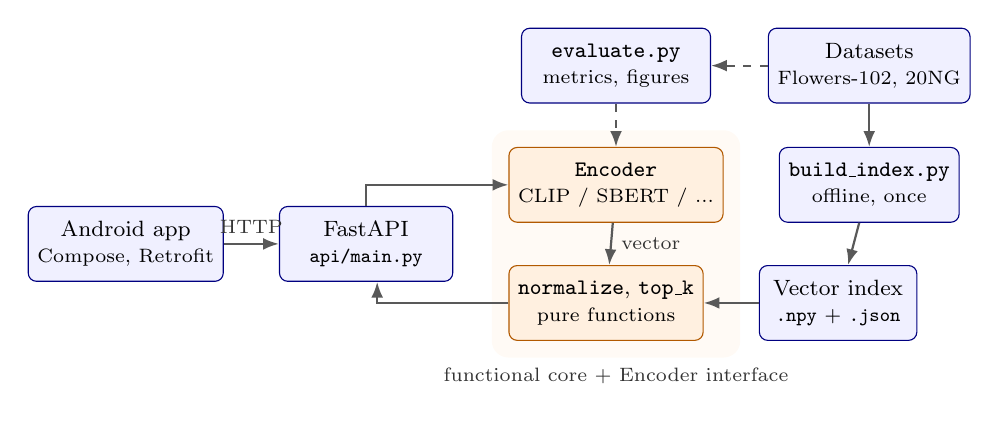
\begin{tikzpicture}[
  box/.style={draw, rounded corners=3pt, minimum height=0.95cm, align=center, font=\footnotesize, fill=white},
  core/.style={box, fill=orange!12, draw=orange!70!black},
  shell/.style={box, fill=blue!6, draw=blue!50!black},
  arr/.style={-{Latex[length=2mm]}, thick, gray!70!black},
  lbl/.style={font=\scriptsize, text=gray!40!black}
]
\node[shell, minimum width=2.2cm] (app) {Android app\\\scriptsize Compose, Retrofit};
\node[shell, minimum width=2.2cm, right=0.7cm of app] (api) {FastAPI\\\scriptsize \texttt{api/main.py}};
\node[core, minimum width=2.4cm, right=0.7cm of api, yshift=0.75cm] (enc) {\texttt{Encoder}\\\scriptsize CLIP / SBERT / ...};
\node[core, minimum width=2.4cm, right=0.7cm of api, yshift=-0.75cm] (search) {\texttt{normalize}, \texttt{top\_k}\\\scriptsize pure functions};
\node[shell, minimum width=2.0cm, right=0.7cm of search] (index) {Vector index\\\scriptsize \texttt{.npy} + \texttt{.json}};
\node[shell, minimum width=2.0cm, right=0.7cm of enc] (build) {\texttt{build\_index.py}\\\scriptsize offline, once};
\node[shell, minimum width=2.0cm, above=0.55cm of build] (data) {Datasets\\\scriptsize Flowers-102, 20NG};
\node[shell, minimum width=2.4cm, above=0.55cm of enc] (eval) {\texttt{evaluate.\allowbreak py}\\\scriptsize metrics, figures};

\draw[arr] (app) -- node[lbl, above]{HTTP} (api);
\draw[arr] (api) |- (enc);
\draw[arr] (enc) -- node[lbl, right]{vector} (search);
\draw[arr] (index) -- (search);
\draw[arr] (search.west) -| ([xshift=4pt]api.south);
\draw[arr] (data) -- (build);
\draw[arr] (build) -- (index);
\draw[arr, dashed] (eval) -- (enc);
\draw[arr, dashed] (data) -- (eval);

\begin{scope}[on background layer]
\node[fill=orange!4, rounded corners=6pt, inner sep=6pt, fit=(enc)(search), label={[lbl]below:functional core + Encoder interface}] {};
\end{scope}
\end{tikzpicture}
\caption{Architecture. Orange boxes are the pure core (the math and the \texttt{Encoder} interface). Blue boxes are the imperative shell that deals with files, the network, and the user. The dataset is encoded once offline; at query time only the query is encoded.}
\label{fig:arch}
\end{figure}

\subsection{Overview}

Figure~\ref{fig:arch} shows the whole system. There are two paths:
\begin{itemize}
  \item \textbf{Offline, once:} \texttt{build\_index.py} loads a dataset, encodes every item, normalizes the vectors, and saves them to disk as a NumPy array plus a JSON file with the labels and paths. This is the slow part (seconds to minutes), and it never runs at query time.
  \item \textbf{Online, per query:} the app sends text or a photo to the API. The API encodes only that one query, normalizes it, takes the dot product with the whole index, and returns the top $k$ with their labels, scores, and image URLs.
\end{itemize}
The same core functions are also used by \texttt{evaluate.\allowbreak py}, which runs every experiment and writes the metrics and figures.

\subsection{Paradigms in the design}

Table~\ref{tab:paradigms} lists where each paradigm shows up and why I picked it for that part. The main idea is that each part of the problem gets the paradigm that fits it best.

\begin{table}[h]
\centering\small
\caption{Which paradigm is used where, and why.}
\label{tab:paradigms}
\begin{tabular}{@{}p{2.5cm}p{3.1cm}p{7cm}@{}}
\toprule
Part & Paradigm & Why it fits \\
\midrule
\texttt{Encoder} and its 4 classes & Object-oriented (polymorphism, Strategy pattern) & The question ``which model?'' is hidden behind one method, \texttt{encode(items)}. Search and evaluation never check the type, so adding a model is one new class. \\
\texttt{search.\allowbreak py}, \texttt{metrics.\allowbreak py} & Functional (pure functions, composition, whole-array operations) & The math has no state. Each function takes arrays and returns new arrays, so it is easy to test with tiny hand-made inputs and to chain: \texttt{search = top\_k} $\circ$ \texttt{normalize} $\circ$ \texttt{encode}. \\
\texttt{evaluate.\allowbreak py}, \texttt{build\_index.py} & Imperative shell & Downloading data, caching vectors, timing, and writing files are side effects. They live at the edge and call the pure core. \\
FastAPI + Pydantic & Declarative & Endpoints and input rules (\texttt{k} between 1 and 100) are declared with types, and the framework does the validation and docs. \\
Upload endpoint, Android & Asynchronous / event-driven & Uploads are awaited with \texttt{async}; the app uses Kotlin coroutines so the UI never blocks on the network. \\
Compose UI + ViewModel & Reactive, declarative UI & The screen is a function of state. When \texttt{results} changes, Compose redraws only what changed. \\
\bottomrule
\end{tabular}
\end{table}

\subsection{Key design decisions}

\begin{itemize}
  \item \textbf{Cosine similarity as a dot product.} Every vector is scaled to length 1 when it enters the index, so cosine similarity becomes a plain dot product. Scoring the whole index is one matrix-vector product, which NumPy does very fast.
  \item \textbf{Exact search first, approximate later.} For 2k to 11k items, exact brute-force search is already fast (Section~\ref{sec:results}), so I kept it as the default because it is simple and always correct. FAISS is measured as the upgrade path for bigger data.
  \item \textbf{Structural interface, not inheritance.} \texttt{Encoder} is a Python \texttt{Protocol}: any object with a \texttt{name} and an \texttt{encode} method counts. This let me pass a 5-line fake encoder in tests without importing PyTorch.
  \item \textbf{Thin client.} The models are hundreds of megabytes, so they stay on the server. The phone only sends the query and shows the results, which keeps the app small. This is the standard setup for this kind of app.
  \item \textbf{Same splits as the dataset authors.} I used the official splits so a query is never in its own database and the results are comparable with other work.
\end{itemize}

%=====================================================================
\section{Implementation}
%=====================================================================

The project is about 1,370 lines: about 800 lines of Python for the engine, evaluation, and API, about 240 lines of tests, and about 310 lines of Kotlin for the app (Table~\ref{tab:files}). I kept the code simple on purpose: short functions, plain names, and no clever tricks.

\begin{table}[h]
\centering\small
\caption{Main files.}
\label{tab:files}
\begin{tabular}{@{}lrp{8.3cm}@{}}
\toprule
File & Lines & What it does \\
\midrule
\texttt{similarity/encoders.py} & 109 & \texttt{Encoder} protocol; CLIP, Sentence-BERT, TF-IDF, color histogram \\
\texttt{similarity/search.py} & 33 & \texttt{normalize}, \texttt{scores}, \texttt{top\_k}, \texttt{search} \\
\texttt{similarity/metrics.py} & 70 & P@$k$, R@$k$, AP, chunked \texttt{evaluate}, per-class AP, confusion \\
\texttt{similarity/data.py} & 51 & Dataset loaders and the 102 flower names \\
\texttt{evaluate.\allowbreak py} & 398 & All experiments, speed tests, CSV/JSON output, figures \\
\texttt{build\_index.py} & 41 & Builds the indexes the API serves \\
\texttt{api/main.py} & 115 & FastAPI app \\
\texttt{tests/} & 239 & 24 tests (metrics, search, encoders, API) \\
\texttt{android/.../*.kt} & 314 & \texttt{MainActivity}, \texttt{SearchViewModel}, \texttt{Api} \\
\bottomrule
\end{tabular}
\end{table}

\subsection{Encoders}

The interface is two lines. Everything else in the system only depends on it:
\begin{lstlisting}[language=Python]
class Encoder(Protocol):
    name: str
    def encode(self, items) -> np.ndarray: ...
\end{lstlisting}
\texttt{ClipEncoder} loads CLIP from Hugging Face Transformers~\cite{wolf2020transformers} on PyTorch~\cite{paszke2019pytorch} and picks CUDA, Apple MPS, or CPU automatically. If the items are strings it runs the text tower, otherwise the image tower, so the same object can do image-to-image, text-to-image, and text-to-text. Images are opened lazily from disk in batches of 64, so the 8,189 photos never sit in memory at once. \texttt{TextEncoder} wraps the \texttt{sentence-transformers} library. \texttt{TfidfEncoder} uses scikit-learn~\cite{pedregosa2011sklearn} and returns a sparse matrix. \texttt{ColorHistogramEncoder} resizes each image to $128\times128$, converts it to HSV, and counts pixels in $8\times8\times8$ color buckets.

\subsection{Search and metrics}

The core of the search is a few lines of NumPy~\cite{harris2020numpy}:
\begin{lstlisting}[language=Python]
def top_k(index, query, k=10):
    s = scores(index, query)
    k = min(k, len(s))
    best = np.argpartition(-s, k - 1)[:k]
    best = best[np.argsort(-s[best])]
    return best, s[best]
\end{lstlisting}
\texttt{argpartition} finds the top $k$ in linear time and only those $k$ get sorted. The metrics work on a boolean ``relevance matrix'' where row $i$ says, for query $i$, whether each ranked result has the right label. Average precision is a cumulative sum divided by the rank, all with whole-array operations:
\begin{lstlisting}[language=Python]
def average_precision(rel, total_relevant):
    hits = np.cumsum(rel, axis=1)
    ranks = np.arange(1, rel.shape[1] + 1)
    return (hits / ranks * rel).sum(axis=1) / np.maximum(total_relevant, 1)
\end{lstlisting}
Because mAP needs the \emph{full} ranking of the database for every query, \texttt{evaluate} processes the queries in chunks of 512 so memory stays small (7,317 queries $\times$ 11,014 posts would otherwise be a 640\,MB rank matrix).

\subsection{API and Android app}

The API is built with FastAPI~\cite{ramirez2018fastapi}. It loads the indexes and models once at startup using FastAPI's lifespan hook and keeps them in a dictionary of \texttt{Collection} objects. Image results include a URL back to the API so the app can load the picture. The Android app follows MVVM: \texttt{SearchViewModel} holds the state (selected collection, query, results, loading, error) as Compose state, and calls the API with Retrofit inside \texttt{viewModelScope}. The photo is picked with the system photo picker, read on the IO dispatcher, and uploaded as multipart form data. Results show in a two-column grid (flowers) or a list of cards (posts), with images loaded by Coil.

\subsection{Problems I ran into}

\begin{itemize}
  \item \textbf{CLIP's 77-token limit.} CLIP's text encoder only reads 77 tokens. Long newsgroup posts crashed it at first, so the tokenizer now truncates to 77 tokens. This also explains part of why CLIP is weaker on long text (Section~\ref{sec:results}).
  \item \textbf{TF-IDF memory.} A dense TF-IDF matrix for 11k posts and 50k words would be over 2\,GB. Keeping it sparse and teaching \texttt{normalize} and \texttt{scores} to accept sparse matrices fixed this without changing the callers.
  \item \textbf{Empty posts.} With headers, footers, and quotes removed (the standard setting, so the model cannot cheat by reading the newsgroup name), 300 train posts and 215 test posts become empty. I drop them from both the database and the queries.
  \item \textbf{Re-encoding is slow.} Encoding is the slow step, so \texttt{evaluate.\allowbreak py} caches every set of vectors to \texttt{cache/} and reuses the image vectors for the text-to-image experiment instead of encoding the photos again.
\end{itemize}

%=====================================================================
\section{Testing, verification, and evaluation}
\label{sec:testing}
%=====================================================================

\subsection{Automated tests}

There are 24 tests run with \texttt{pytest}, and none of them need a GPU or a model download (NFR5), so they run in under 2 seconds.
\begin{itemize}
  \item \textbf{Metrics, checked by hand (8 tests).} For a ranking \texttt{[hit, miss, hit, miss]} with 2 relevant items, AP must be $(1/1 + 2/3)/2$. Missed relevant items must lower AP. Perfectly separated clusters must give mAP $= 1$. Random vectors with 10 classes must give P@10 close to the chance level of 0.1. Splitting queries into chunks must not change any number.
  \item \textbf{Search and encoders (7 tests).} Normalized vectors have length 1, zero vectors do not produce NaN, \texttt{top\_k} returns results in the right order, asking for more results than items works, TF-IDF works through the sparse path, and the color histogram matches a red image to a red image.
  \item \textbf{API (9 tests).} Using FastAPI's test client and a fake encoder, the tests check every endpoint, including the error cases: unknown collection (404), \texttt{k = 0} or empty text (422), a text file uploaded as an image (400), and an image search on the text collection (400).
\end{itemize}
Before running anything on a GPU, I also ran \texttt{evaluate.\allowbreak py} end to end with fake datasets and fake encoders to make sure every experiment, table, and figure is produced without errors.

\subsection{Experiment setup}

I compared these methods (none of them is trained):
\begin{itemize}
  \item \textbf{Images:} color histogram (baseline), CLIP ViT-B/32, CLIP ViT-L/14.
  \item \textbf{Text:} TF-IDF (baseline), \texttt{all-MiniLM-L6-v2}, \texttt{all-mpnet-base-v2}, and CLIP ViT-B/32's text tower (to test the ``swap the model'' claim, NFR2).
  \item \textbf{Text-to-image:} CLIP ViT-B/32 and ViT-L/14 with 102 prompts.
  \item \textbf{Speed:} per-query latency for NumPy exact search, FAISS flat (exact), and FAISS HNSW (approximate, $M=32$, efSearch $=64$) on the real indexes and on random 512-dimensional indexes with 10k, 50k, and 200k vectors. For HNSW I also report the overlap between its top 10 and the exact top 10.
\end{itemize}
Everything ran in one Google Colab session on an NVIDIA Tesla T4 GPU with Python 3.13, PyTorch 2.14, Transformers 5.22, sentence-transformers 5.7, and FAISS 1.16. The search speed tests run on the Colab CPU. The full run, including downloading the models and datasets, took 23.8 minutes. After dropping empty posts, 20 Newsgroups has 11,014 train posts (database) and 7,317 test posts (queries).

%=====================================================================
\section{Results, discussion, and limitations}
\label{sec:results}
%=====================================================================

\subsection{Main results}

Table~\ref{tab:main} has the main numbers and Figure~\ref{fig:pk} shows Precision@$k$ for every method. For reference, picking results at random would give P@10 of about 0.01 on Flowers-102 (20 right answers out of 2,040) and about 0.05 on 20 Newsgroups (20 topics).

\begin{table}[h]
\centering\small
\caption{Main results. No method is trained. Best per task in bold. Flowers-102 queries: 6,149 test photos against 2,040 database photos. 20 Newsgroups: 7,317 test posts against 11,014 train posts. Text-to-image: 102 prompts against all 8,189 photos.}
\label{tab:main}
\begin{tabular}{@{}llcccc@{}}
\toprule
Task & Method & P@1 & P@10 & R@100 & mAP \\
\midrule
Image $\rightarrow$ image & Color histogram (baseline) & 0.321 & 0.184 & 0.274 & 0.131 \\
 & CLIP ViT-B/32 & 0.892 & 0.731 & 0.834 & 0.616 \\
 & CLIP ViT-L/14 & \textbf{0.980} & \textbf{0.917} & \textbf{0.944} & \textbf{0.836} \\
\midrule
Text $\rightarrow$ text & TF-IDF (baseline) & 0.565 & 0.469 & 0.057 & 0.142 \\
 & MiniLM-L6 (Sentence-BERT) & 0.673 & 0.588 & 0.084 & 0.290 \\
 & MPNet-base (Sentence-BERT) & \textbf{0.697} & \textbf{0.623} & \textbf{0.091} & \textbf{0.325} \\
 & CLIP ViT-B/32 text tower & 0.552 & 0.474 & 0.060 & 0.169 \\
\midrule
Text $\rightarrow$ image & CLIP ViT-B/32 & 0.735 & 0.689 & 0.606 & 0.571 \\
 & CLIP ViT-L/14 & \textbf{0.814} & \textbf{0.794} & \textbf{0.761} & \textbf{0.748} \\
\bottomrule
\end{tabular}
\end{table}

\begin{figure}[h]
\centering
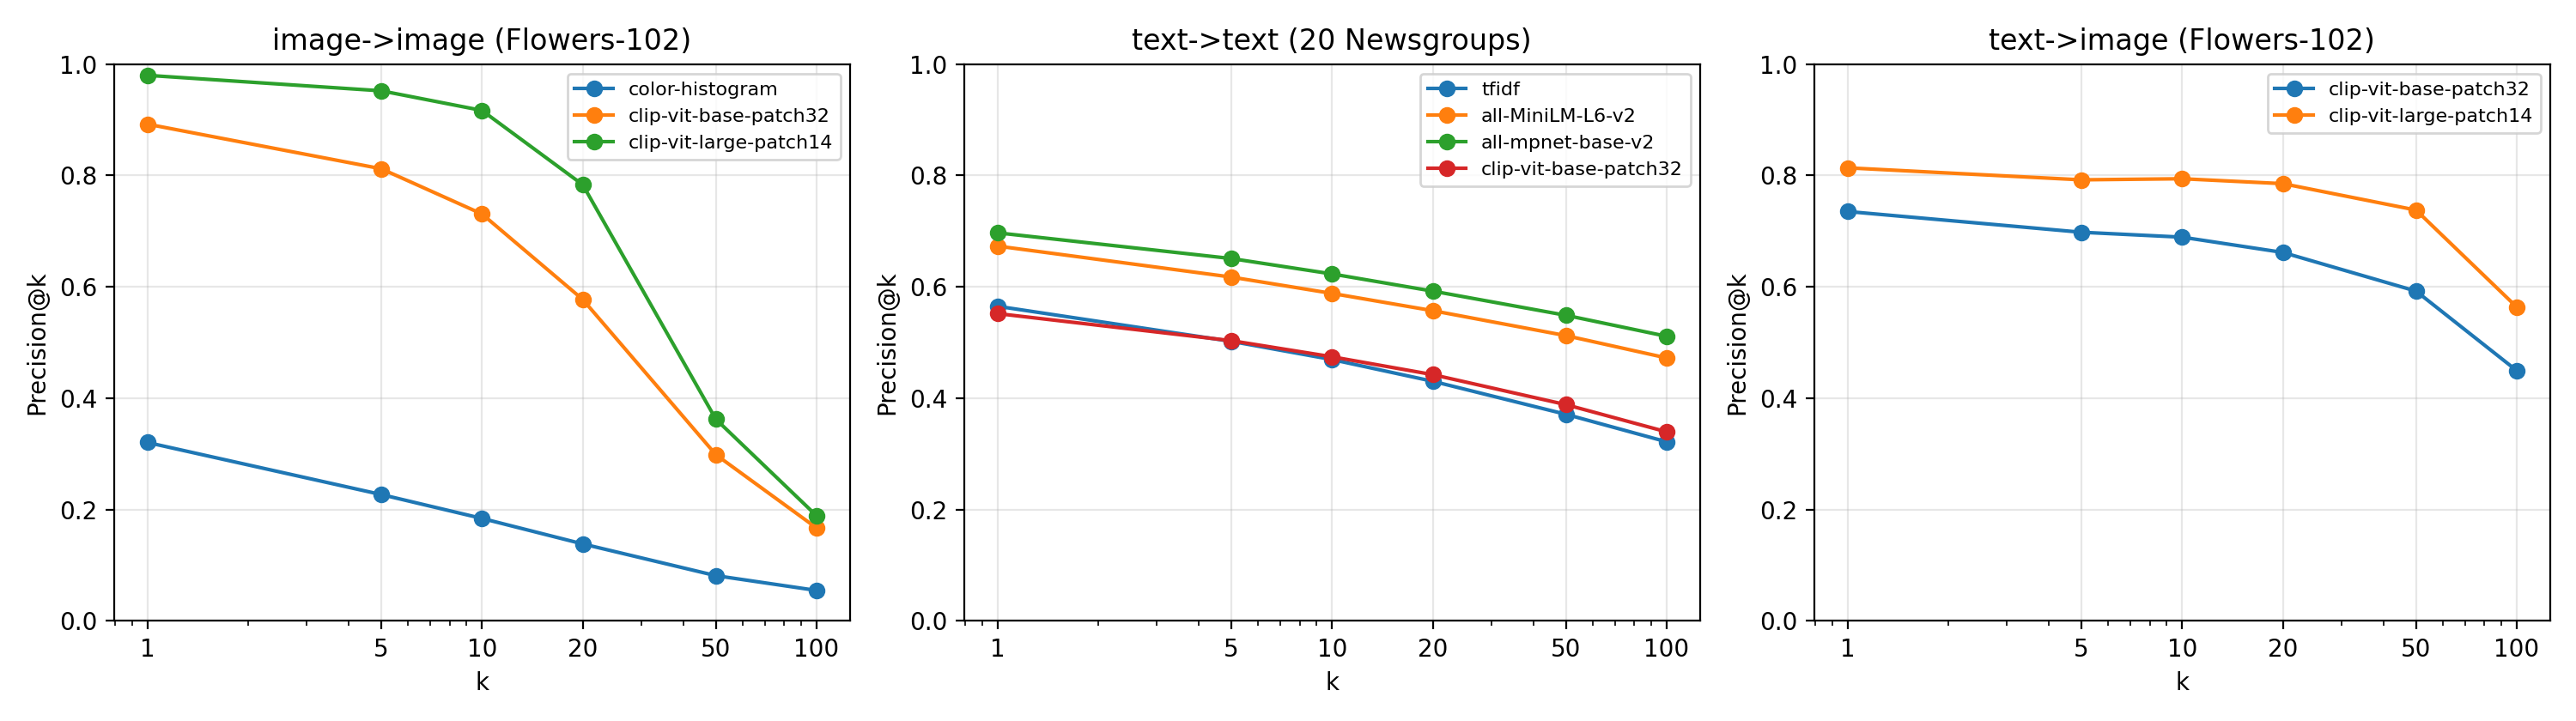
\includegraphics[width=\linewidth]{figures/precision_at_k.png}
\caption{Precision@$k$ for every method. On Flowers-102 each query has exactly 20 right answers, which is why every curve drops after $k=20$.}
\label{fig:pk}
\end{figure}

\paragraph{Images.} This is where the idea works best. CLIP ViT-B/32 already returns a correct species as the top result 89\% of the time, and ViT-L/14 does it 98\% of the time. Both are far ahead of the color histogram, which only gets the top result right 32\% of the time: many flowers share colors (there are a lot of yellow and pink species), so color alone is not enough. Figure~\ref{fig:examples} shows real queries. The results match in species, not just in color: the purple and the pink morning glories are both found for a blue morning glory query.

\begin{figure}[h]
\centering
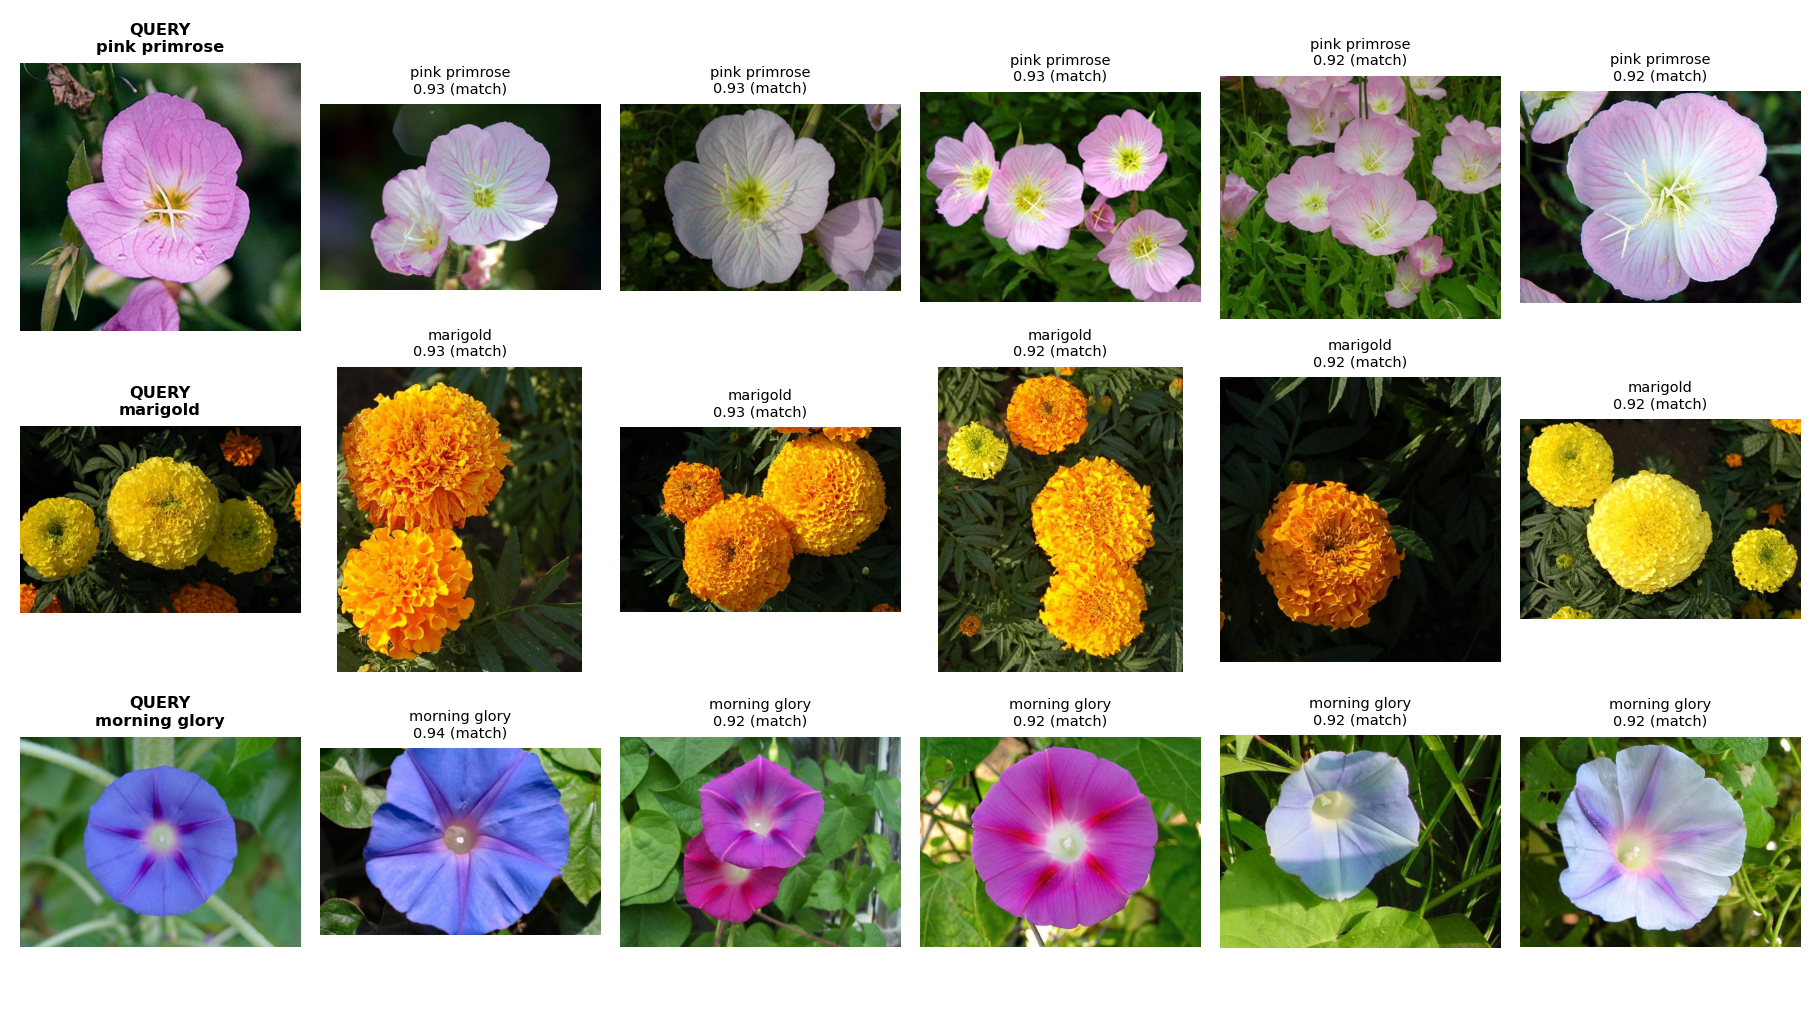
\includegraphics[width=0.93\linewidth]{figures/example_image_search.png}
\caption{Image-to-image search with CLIP ViT-B/32. Left: the query photo. Right: the top 5 results from the database with their cosine similarity. All 15 results are the right species.}
\label{fig:examples}
\end{figure}

\paragraph{Text.} Both Sentence-BERT models beat TF-IDF on every metric. MPNet is the best (P@10 = 0.62, mAP = 0.33), and the small MiniLM is close behind (0.59 and 0.29). The mAP values for text look low next to the images, but that is because of how the task is built: every query has around 550 correct posts in the database (all the posts from the same newsgroup), and AP only gets high if \emph{all} of them are ranked near the top. For a user who only looks at the first 10 results, P@10 is the more useful number, and there about 6 of the top 10 posts are from the same newsgroup.

\paragraph{Text-to-image.} The same CLIP image index, with no changes, also answers text queries. Typing ``a photo of a tiger lily, a type of flower.'' returns the right flower first for 81\% of the 102 species with ViT-L/14. Figure~\ref{fig:t2i} shows three examples. I find this the most impressive result, because the system never saw a labeled flower photo.

\begin{figure}[h]
\centering
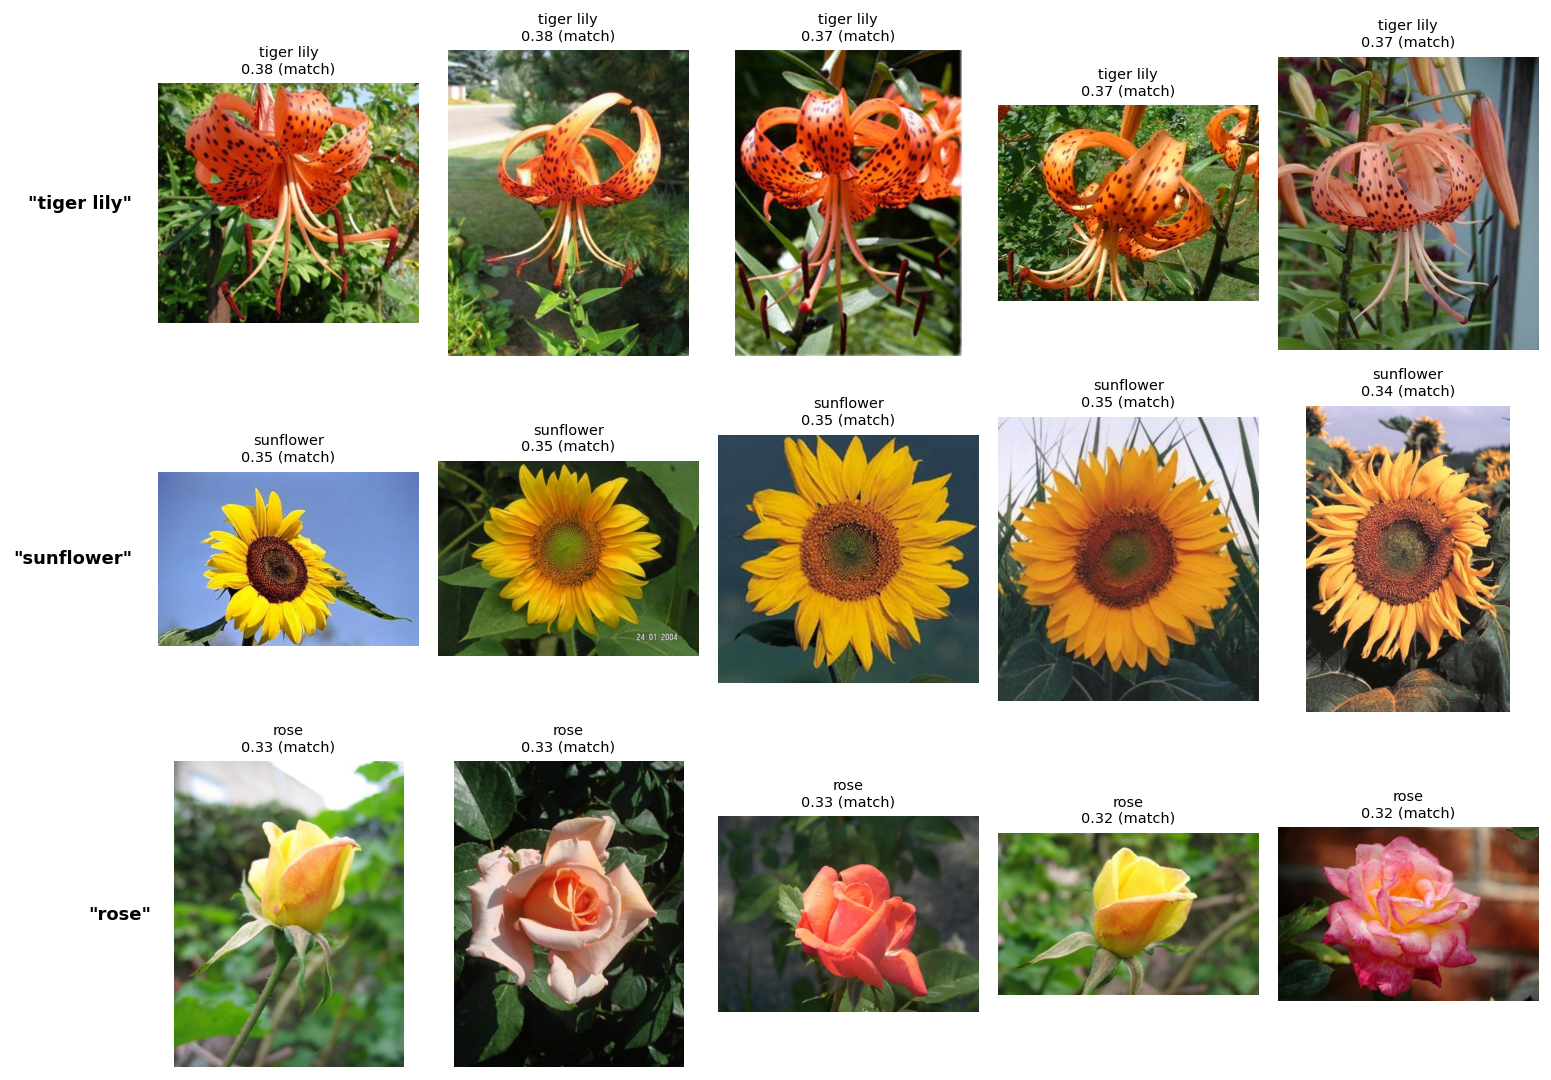
\includegraphics[width=0.85\linewidth]{figures/example_text_to_image.png}
\caption{Text-to-image search with CLIP ViT-B/32. Each row is a typed query and its top 5 photos out of 8,189.}
\label{fig:t2i}
\end{figure}

\subsection{Swapping the model}

The ``CLIP text tower'' row in Table~\ref{tab:main} came from adding one line to the list of encoders, with no changes to the search or metrics code (NFR2). The result itself is useful too: CLIP is only about as good as TF-IDF on newsgroup posts (mAP 0.17 versus 0.14). CLIP was trained on short image captions and only reads the first 77 tokens, so it is the wrong tool for long forum posts. The design makes it cheap to find this out, which is the point of keeping the model behind an interface.

\subsection{Where it fails}

\paragraph{Similar topics get mixed up.} Figure~\ref{fig:confusion} shows, for each query topic, which topic the closest post came from. Most mistakes are between topics that really overlap: 28\% of \texttt{talk.\allowbreak religion.\allowbreak misc} queries land on \texttt{soc.\allowbreak religion.\allowbreak christian}, 25\% of \texttt{talk.\allowbreak politics.\allowbreak misc} land on \texttt{talk.\allowbreak politics.\allowbreak guns}, and Mac and PC hardware get mixed up 13\% of the time. When the query is a computer topic, the closest post is from \emph{some} computer topic 87\% of the time. The easiest topics are the two sports groups (hockey 91\% and baseball 83\% top-1), which have very distinct vocabulary.

\begin{figure}[h]
\centering
\begin{subfigure}[t]{0.52\linewidth}
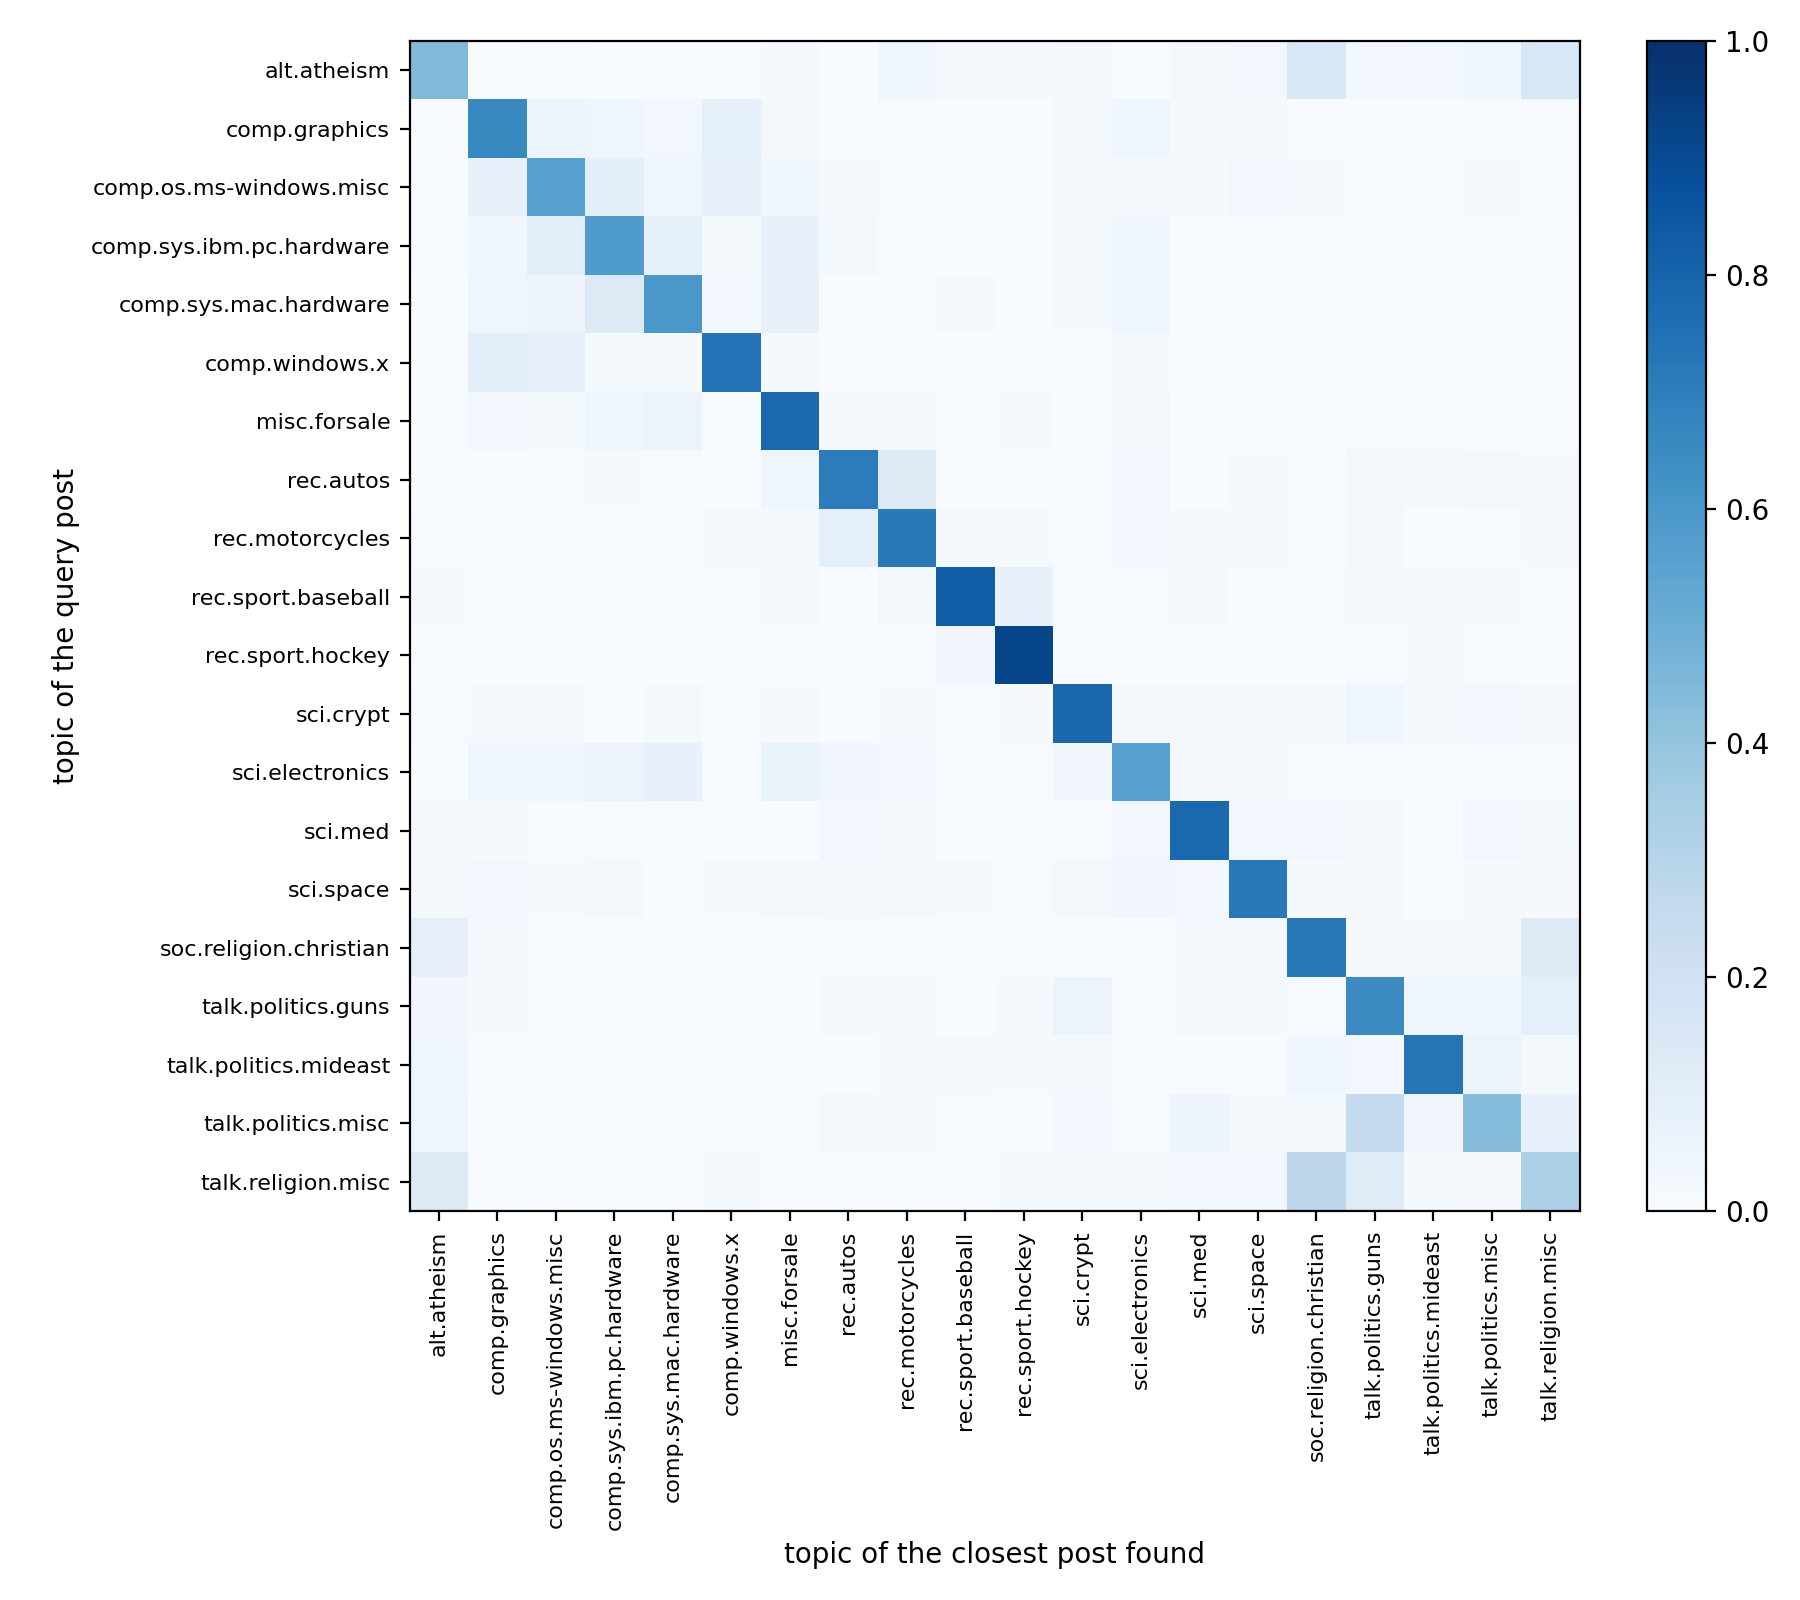
\includegraphics[width=\linewidth]{figures/news_confusion.png}
\caption{Top-1 confusion (MiniLM), row-normalized.}
\label{fig:confusion}
\end{subfigure}\hfill
\begin{subfigure}[t]{0.46\linewidth}
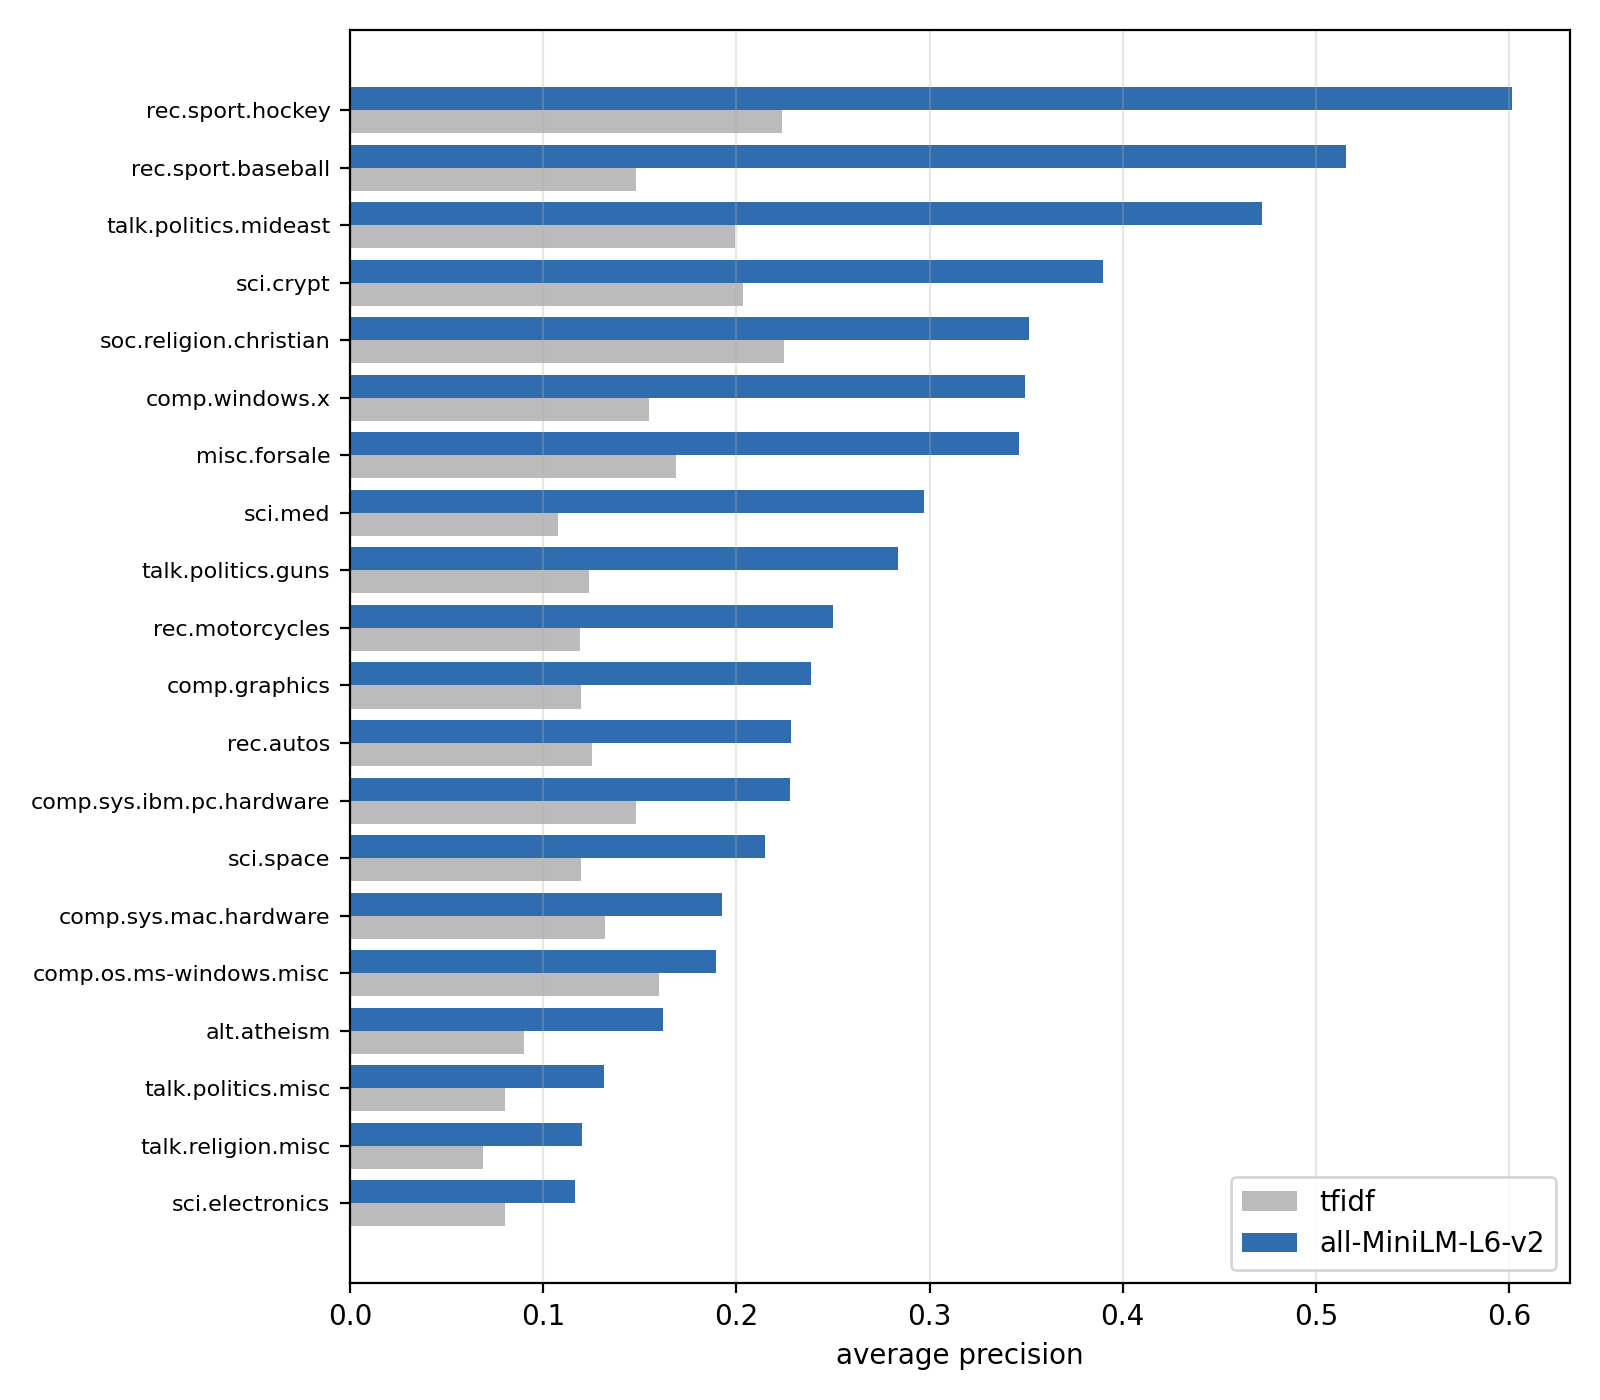
\includegraphics[width=\linewidth]{figures/news_ap_by_topic.png}
\caption{AP per topic, MiniLM versus TF-IDF.}
\label{fig:topics}
\end{subfigure}
\caption{Error analysis on 20 Newsgroups. MiniLM beats TF-IDF on all 20 topics.}
\end{figure}

\paragraph{Labels are not the same as meaning.} Table~\ref{tab:qual} shows four typed queries. For ``should I take antibiotics for a cold'', TF-IDF's top result comes from \texttt{talk.\allowbreak politics.\allowbreak guns} (it matched on common words), while MiniLM returns three \texttt{sci.\allowbreak med} posts. But for ``my graphics card driver keeps crashing'', TF-IDF gets the \texttt{comp.\allowbreak graphics} label right just by matching the word ``graphics'', while MiniLM returns Windows and PC hardware posts. Those posts are arguably \emph{more} useful for a crashing driver, but they count as wrong. So label-based metrics sometimes underrate semantic search.

\begin{table}[h]
\centering\small
\caption{Topics of the top 3 results for typed queries (database: 20 Newsgroups train).}
\label{tab:qual}
\begin{tabular}{@{}p{4.1cm}p{4.3cm}p{4.3cm}@{}}
\toprule
Query & TF-IDF & MiniLM \\
\midrule
NASA is planning a new mission to send astronauts to Mars & sci.space, sci.space, sci.space & sci.space, sci.space, sci.space \\
my graphics card driver keeps crashing when I render 3D scenes & comp.graphics $\times$3 & ms-windows.misc $\times$2, ibm.pc.hardware \\
should I take antibiotics for a cold & \textbf{politics.guns}, sci.med, sci.med & sci.med, sci.med, sci.med \\
who will win the world series this year & baseball, \textbf{hockey}, baseball & baseball, baseball, baseball \\
\bottomrule
\end{tabular}
\end{table}

\paragraph{Hard flower classes.} The per-class AP for CLIP ViT-B/32 ranges from 0.15 (canterbury bells) to 0.997 (cautleya spicata), with a median of 0.64 (Figure~\ref{fig:flowerclasses} in the appendix). The hardest classes are ones that look alike or vary a lot inside the class: canterbury bells, sword lily, carnation, and petunia come in many colors, and several purple bell-shaped species get confused with each other.

\subsection{Speed}

\begin{table}[h]
\centering\small
\caption{Encoding speed on a T4 GPU (items per second) and per-query search time on the Colab CPU (ms, $k=10$). HNSW overlap is how many of the exact top 10 it also returns.}
\label{tab:speed}
\begin{tabular}{@{}lr@{\hspace{2em}}lrrrr@{}}
\toprule
Encoder & items/s & Index & NumPy & FAISS flat & HNSW & overlap \\
\midrule
Color histogram & 155 & Flowers, 2,040 $\times$ 512 & 1.64 & 0.21 & 0.15 & 1.000 \\
CLIP ViT-B/32 (images) & 118 & 20NG, 11,014 $\times$ 384 & 0.85 & 0.74 & 0.18 & 0.995 \\
CLIP ViT-L/14 (images) & 18 & random, 10k $\times$ 512 & 1.10 & 0.92 & 0.47 & -- \\
TF-IDF & 7,987 & random, 50k $\times$ 512 & 7.42 & 7.78 & 1.05 & -- \\
MiniLM-L6 & 379 & random, 200k $\times$ 512 & 31.9 & 35.2 & 1.14 & -- \\
MPNet-base & 60 & & & & & \\
\bottomrule
\end{tabular}
\end{table}

Table~\ref{tab:speed} and Figure~\ref{fig:latency} (appendix) show the speed results. Exact NumPy search over the real indexes takes under 2\,ms per query, far under the 100\,ms target (NFR3). (The 1.64\,ms for the smaller Flowers index is higher than the 0.85\,ms for the bigger 20NG index because it was the first test to run, so it includes warm-up.) Exact search grows linearly: about 32\,ms at 200k vectors. FAISS HNSW stays around 1\,ms even at 200k, and on the real indexes it returns 99.5--100\% of the exact top 10. On the random vectors its overlap is low, which is expected: random high-dimensional points have no neighborhood structure for the graph to follow, so I only report overlap on real data. HNSW also costs build time (158\,s for 200k vectors). For this project's sizes, exact search is the right choice, and HNSW is the upgrade if the index grows past about 50k items.

The real cost is encoding. ViT-L/14 is 6.6$\times$ slower than ViT-B/32 and MPNet is 6.3$\times$ slower than MiniLM. For images the bigger model is worth it (+22 mAP points), but for text MiniLM gives most of the quality (+15 points over TF-IDF versus +18 for MPNet) at 6 times the speed. That is why the API uses MiniLM for text. It uses ViT-B/32 for images so it can run on a laptop CPU. Switching to ViT-L/14 only means changing the model name in \texttt{build\_index.py} and \texttt{api/main.py}.

\subsection{Limitations}

\begin{itemize}
  \item \textbf{Relevance is ``same label''.} This is easy to measure but rough. As Table~\ref{tab:qual} shows, a result can be useful and still count as wrong, and the opposite can happen too.
  \item \textbf{Only two datasets, each fairly clean.} Flowers-102 photos are centered and well lit, and 20 Newsgroups is from the 1990s. Real user photos and modern text would probably score lower.
  \item \textbf{Long text gets cut.} CLIP reads 77 tokens and MiniLM reads 256 word pieces, so the end of long posts is ignored.
  \item \textbf{One run, one machine.} No training means the metrics do not change between runs, but the speed numbers are from one Colab machine and would be different on other hardware.
  \item \textbf{The app and API are a demo.} The Android app has no automated tests, and the API has no authentication or rate limiting, so it is not a production service.
\end{itemize}

%=====================================================================
\section{Software process and teamwork}
%=====================================================================

I did this project alone, so ``teamwork'' here means how I organized my own work. I followed the plan from my proposal in small steps and kept a working version at every step:
\begin{enumerate}
  \item \textbf{Proposal.} Picked the idea, the datasets, and the metrics, and wrote the proposal in the NeurIPS format.
  \item \textbf{Prototype and check-in (October 22).} A single Colab notebook with the \texttt{Encoder} class, the pure functions, and metrics on small subsets (10 flower species and 5 topics). This notebook is kept in the repo as \texttt{checkin\_prototype.ipynb}.
  \item \textbf{Engine and tests (November).} Moved the notebook code into a Python package with unit tests (the metrics are the easiest place to make a silent mistake, so they got the most tests), then added the baselines and the full evaluation script.
  \item \textbf{API and app (November).} Built the FastAPI service on top of the same package, then the Android client on top of the API.
  \item \textbf{Final run and report (late November).} Ran everything once on a GPU and wrote the report from the saved results.
\end{enumerate}
I used Git and GitHub for version control and Google Colab for GPU time. The biggest process lesson was to build the evaluation early: once the metrics were tested, every later change could be checked with real numbers instead of by looking at a few examples.

%=====================================================================
\section{Reproducibility and artifacts}
%=====================================================================

Everything is in the public repository \url{https://github.com/al3j4ndrolm/similarity-cs152}:
\begin{itemize}
  \item \textbf{One-click run.} \texttt{notebooks/run\_everything.ipynb} clones the repo, installs the requirements, runs the tests, runs \texttt{evaluate.\allowbreak py}, shows the figures, and downloads \texttt{results.\allowbreak zip}. It took 23.8 minutes on a free Colab T4 GPU.
  \item \textbf{Command line.} \texttt{pip install -r requirements.txt}, then \texttt{python evaluate.py}. \texttt{--quick} uses 1 in 20 queries for a fast check, and \texttt{--skip-large} skips the two big models.
  \item \textbf{Saved results.} \texttt{results/} has every table as CSV (\texttt{metrics.\allowbreak csv}, \texttt{search\_speed.csv}, \texttt{encode\_speed.csv}, per-class and per-topic AP, and the confusion matrix), a \texttt{summary.\allowbreak json} with the software versions and GPU, and all figures.
  \item \textbf{Determinism.} No training means no random seeds affect the metrics. The datasets use their official splits, the models are pinned by name, and the only random numbers (the synthetic speed test) use seed 0. Latency numbers depend on the machine.
  \item \textbf{Demo.} \texttt{python build\_index.py} then \texttt{uvicorn api.main:app}, and open the \texttt{android/} folder in Android Studio.
\end{itemize}

%=====================================================================
\section{Conclusion}
%=====================================================================

The question was whether a useful ``find similar'' engine can be built with no training. For images and text-to-image the answer is clearly yes: CLIP turns a few lines of search code into a system that finds the right flower 98\% of the time and understands typed descriptions of photos it was never trained on. For text the answer is yes with a caveat: Sentence-BERT clearly beats the classic baseline, but topics that overlap in meaning stay hard, and label-based metrics do not always agree with what a person would call similar.

On the paradigms side, the split between an object-oriented \texttt{Encoder} interface, a functional core, and an imperative shell paid off in practice. Adding a baseline or swapping a model never touched the search or evaluation code, the core was easy to test without any model, and the same functions run in the experiments, the API, and (through the API) the Android app.

Next steps would be hybrid search (combining TF-IDF and embeddings, since they fail on different queries), an HNSW index for larger collections, running a small embedding model directly on the phone, and a small user study to measure ``similar'' beyond class labels.

\bibliographystyle{plainnat}
\bibliography{refs}

\appendix
\section{Appendix: extra figures and API example}

\begin{figure}[h]
\centering
\begin{subfigure}[t]{0.5\linewidth}
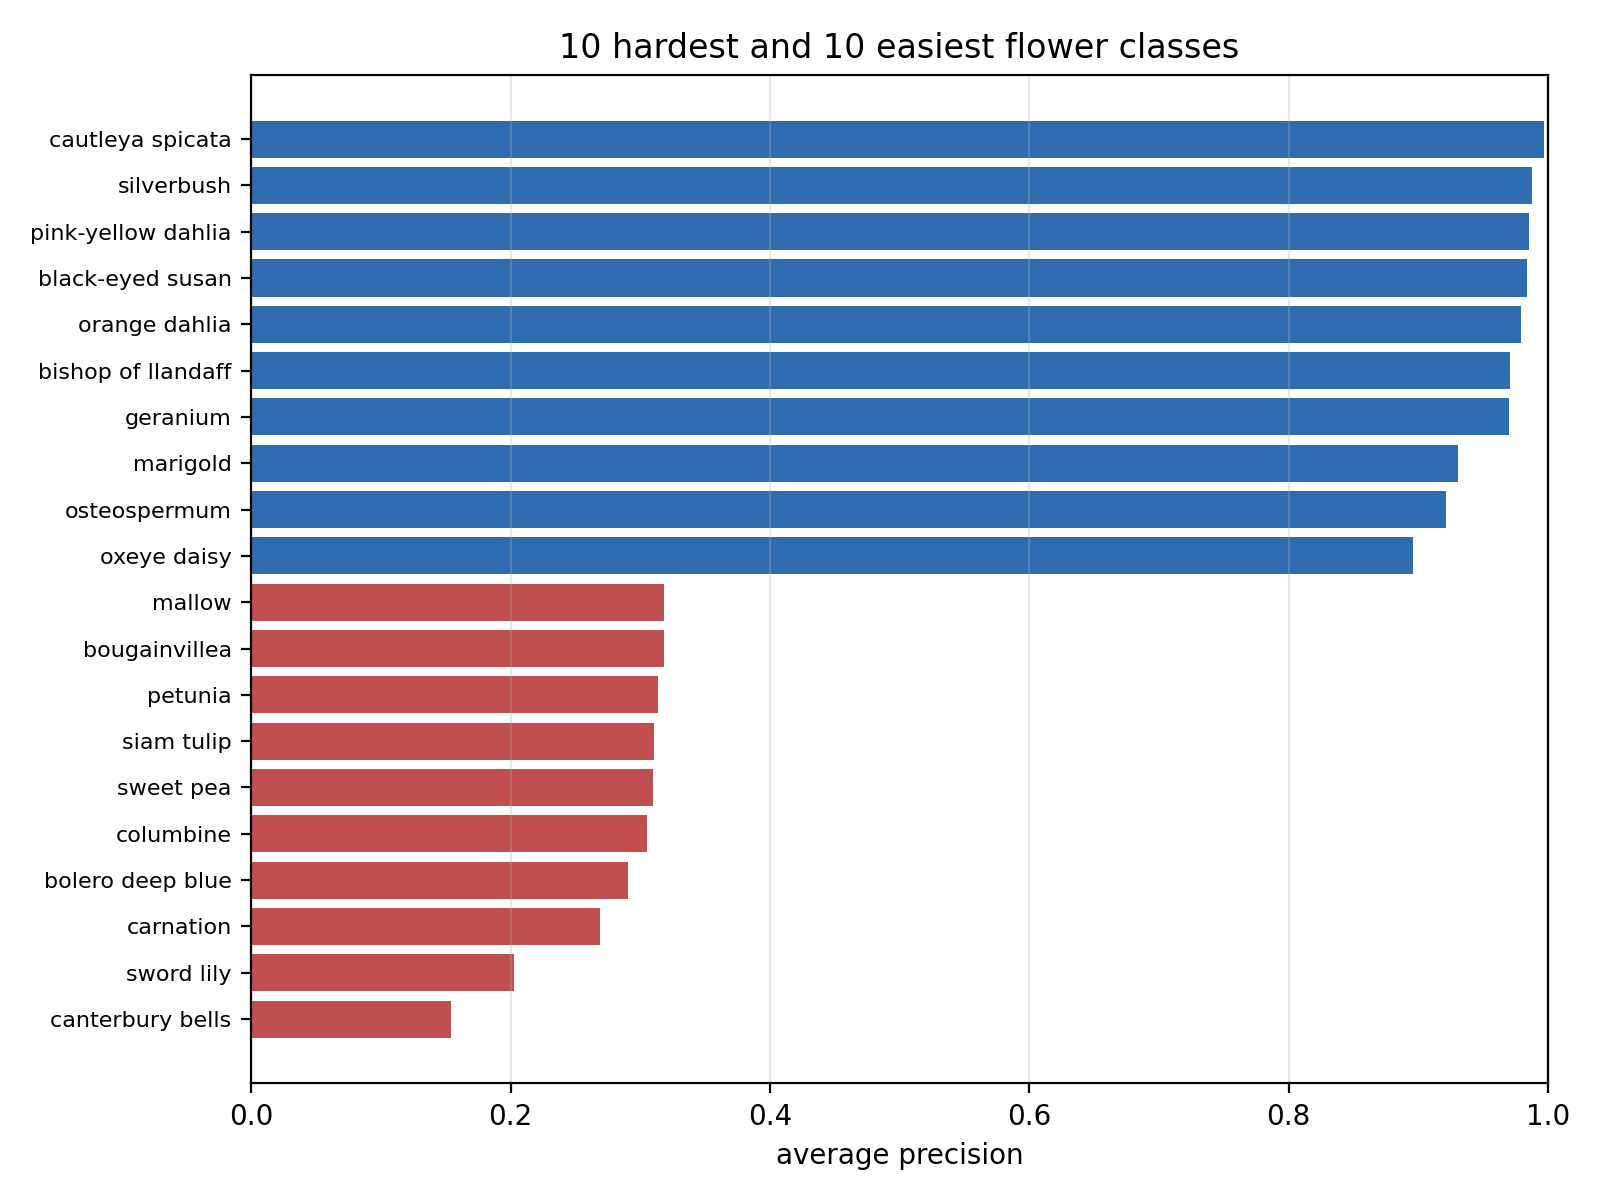
\includegraphics[width=\linewidth]{figures/flowers_ap_by_class.png}
\caption{Hardest and easiest flower classes (CLIP ViT-B/32).}
\label{fig:flowerclasses}
\end{subfigure}\hfill
\begin{subfigure}[t]{0.47\linewidth}
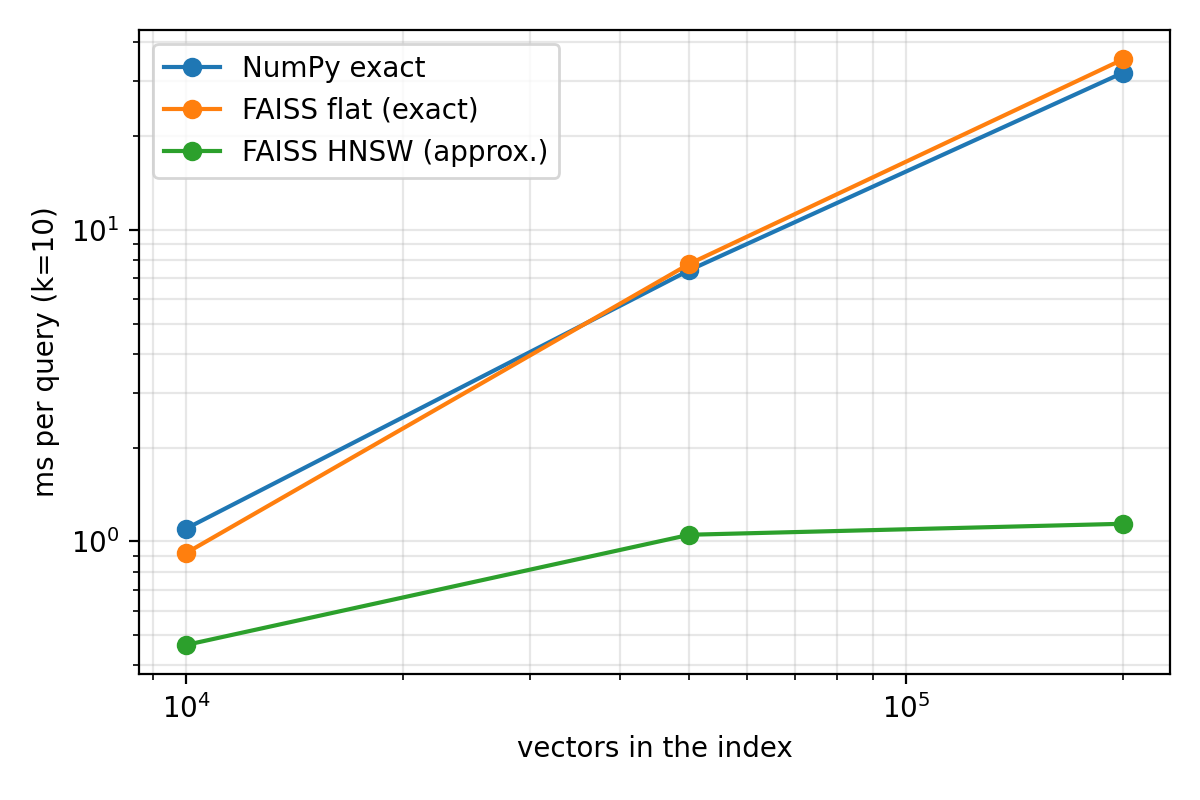
\includegraphics[width=\linewidth]{figures/search_latency.png}
\caption{Search time versus index size (random 512-d vectors).}
\label{fig:latency}
\end{subfigure}
\caption{Per-class quality and search speed.}
\end{figure}

\paragraph{Example API call.}
\begin{lstlisting}
POST /search/text
{"collection": "news", "text": "who will win the world series this year", "k": 2}

{"collection": "news", "count": 2, "results": [
  {"id": 812, "label": "rec.sport.baseball", "score": 0.604, "text": "..."},
  {"id": 4471, "label": "rec.sport.baseball", "score": 0.574, "text": "..."}]}
\end{lstlisting}
The \texttt{id} values above are only illustrative. The scores are the real MiniLM scores from Table~\ref{tab:qual}'s last query.

\paragraph{All metrics.} The file \texttt{results/\allowbreak metrics.csv} in the repository has P@$k$ and R@$k$ for $k \in \{1, 5, 10, 20, 50, 100\}$ and mAP for every row of Table~\ref{tab:main}.

\end{document}
